\documentclass{beamer}

\usetheme{metropolis}
\usefonttheme{serif}
\setbeameroption{hide notes}
\setbeamercolor{note page}{bg=white}
\setbeamercolor{note title}{bg=white}
\setbeamertemplate{bibliography item}{}

\usepackage{fontspec}
\setmainfont{Noto Serif}
\setsansfont{Noto Sans}
\setmonofont{Noto Mono}
\newfontfamily{\cyrillicfont}{Noto Serif}
\newfontfamily{\cyrillicfonttt}{Noto Mono}
\usepackage{microtype}

\usepackage{polyglossia}
\setmainlanguage{english}
\setotherlanguage{russian}

\usepackage{csquotes}
\usepackage{graphicx}
\usepackage{ragged2e}
\usepackage[backend=biber,sorting=none]{biblatex}

% Remove last dot from biblatex entries
\renewcommand{\finentrypunct}{}
% Replace dot between title and url with colon
\renewcommand{\newunitpunct}{\addcolon\space}
% Remove URL prefix from url
\DeclareFieldFormat{url}{\url{#1}}
\addbibresource{bibliography.bib}

\usepackage{hyperref}
\hypersetup{breaklinks=true,unicode=true,pdfencoding=auto}

\usepackage{shellesc}
\usepackage[outputdir=build]{minted}
\setminted{autogobble,fontsize=\scriptsize}


\author{Андрей Лапшин}
\date{2018-04-03}
\title{Привет, мир!\\Локализация Андроид-приложений.
}

\begin{document}
\begin{frame}
    \titlepage
    \note{
        Всем привет. Меня зовут Андрей Лапшин и мой доклад посвящен локализации Android-приложений.
    }
\end{frame}

\begin{frame}
    \frametitle{Что такое локализация?}
    \begin{itemize}
        \item \textbf{Локализация (L10N)} - адаптация приложения для поддержки
            языковых, культурных и других требований определенной страны.
        \item \textbf{Интернационализация (I18N)} - подготовка продукта для
            упрощения процесса локализации
        \item Локализация != Интернационализация
    \end{itemize}
\end{frame}

\begin{frame}
    \frametitle{Для чего нужна локализация?}
    \begin{itemize}
        \item Доступ к более широкой аудитории
        \item Конкурентное преимущество по сравнению с другими продуктами
        \item В процессе интернационализации/локализации улучшается структура проекта
    \end{itemize}
\end{frame}

\begin{frame}
    \frametitle{Типичные проблемы}
    \begin{itemize}
        \item Текст в коде
        \item Конкатенация строк
        \item Форматирование числительных
        \item Форматирование чисел, дат и т. п.
        \item Стилизация строк (курсив, подчеркивание и т. п.)
        \item Фиксированный размер UI-элементов
        \item Текст в изображениях
    \end{itemize}
\end{frame}

\begin{frame}[fragile]
    \frametitle{Текст в коде}
    \begin{minted}{xml}
        <TextView
            android:id="@+id/username"
            android:layout_width="wrap_content"
            android:layout_height="wrap_content"
            android:text="Username"/>
    \end{minted}
\end{frame}

\begin{frame}[fragile]
    \frametitle{Текст в коде}
    \begin{minted}{xml}
        <string name="username">Username</string>
    \end{minted}
    \begin{minted}{xml}
        <TextView
            android:id="@+id/username"
            android:layout_width="wrap_content"
            android:layout_height="wrap_content"
            android:text="@string/username"/>
    \end{minted}
\end{frame}

\begin{frame}[fragile]
    \frametitle{Конкатенация строк}
    \begin{minted}{java}
        greetingTextView.setText(
            "How are you today, " + username);
    \end{minted}
    \begin{minted}{java}
        greetingTextView.setText(
            getString(R.string.greeting) + username);
    \end{minted}
\end{frame}

\begin{frame}[fragile]
    \frametitle{Форматирование строк}
    \begin{minted}{xml}
        <string name="greeting">How are you today, %1$s</string>
    \end{minted}
    \begin{minted}{java}
        greetingTextView.setText(
            getString(R.string.greeting, username));
    \end{minted}
\end{frame}

\begin{frame}[fragile]
    \frametitle{Форматирование строк с использованием Phrase}
    \begin{minted}{xml}
        <string name="greeting">How are you today, {username}</string>
    \end{minted}
    \begin{minted}{java}
        CharSequence greeting = Phrase.from(getString(R.string.greeting))
            .put("username", username)
            .format();
        greetingTextView.setText(greeting);
    \end{minted}
\end{frame}

\begin{frame}
    \frametitle{Форматирование числительных}
    \begin{block}{Английский}
        \begin{itemize}
            \item \textquote{You have 1 new message}
            \item \textquote{You have 10 new messages}
        \end{itemize}
    \end{block}
    \begin{block}{Русский}
        \begin{itemize}
            \item \textquote{У вас 1 новое сообщение}
            \item \textquote{У вас 3 новых сообщения}
            \item \textquote{У вас 10 новых сообщений}
            \item \textquote{У вас 21 новое сообщений}
        \end{itemize}
    \end{block}
\end{frame}

\begin{frame}[fragile]
    \frametitle{Форматирование числительных}
    \texttt{\footnotesize values/strings.xml}
    \begin{minted}{xml}
        <plurals name="new_messages">
            <item quantity="one">You have %d new message</item>
            <item quantity="other">You have %d new messages</item>
        </plurals>
    \end{minted}
    \texttt{\footnotesize values-ru/strings.xml}
    \begin{minted}{xml}
        <plurals name="new_messages">
            <item quantity="one">У вас %d новое сообщение</item>
            <item quantity="few">У вас %d новых сообщения</item>
            <item quantity="other">У вас %d новых сообщений</item>
        </plurals>
    \end{minted}
    \begin{minted}{java}
        int count = getNumberOfNewMessages();
        String newMessages = getResources().getQuantityString(
            R.plurals.new_messages, count, count);
    \end{minted}
\end{frame}

\begin{frame}[fragile]
    \frametitle{Форматирование чисел}
    В зависимости от локали вещественные числа используют разный символ для
    разделения дробной и целой части.
    \begin{minted}{java}
        String piStringImplicit = String.format("%1.2f", Math.PI);
        String piStringExplicit = String.format(Locale.getDefault(), "%1.2f",
            Math.PI);
        String piStringDifferentLocale = String.format(Locale.US, "%1.2f",
            Math.PI);
    \end{minted}
\end{frame}

\begin{frame}[fragile]
    \frametitle{Форматирование дат}
    В зависимости от локали форматирование дат также может отличаться.
    \begin{minted}{java}
        LocalDate date = LocalDate.now();
        DateTimeFormatter formatter1 =
            DateTimeFormatter.ofPattern("MM dd yyyy");
        String dateAsText1 = date.format(formatter1);

        DateTimeFormatter formatter2 =
            DateTimeFormatter.ofPattern(getString(R.string.datetime_format));
        String dateAsText2 = date.format(formatter2);

        DateTimeFormatter formatter3 =
            DateTimeFormatter.ofLocalizedDate(FormatStyle.FULL);
        String dateAsText2 = date.format(formatter3);
    \end{minted}
\end{frame}

\begin{frame}[fragile]
    \frametitle{Spannables}
    \begin{minted}{java}
        SpannableString spannable = new SpannableString("Text styling");
        spannable.setSpan(ForegroundColorSpan(Color.PINK),
            0, 4, Spannable.SPAN_EXCLUSIVE_EXCLUSIVE);
        spanTextView.setText(spannable);
    \end{minted}
    \begin{center}
        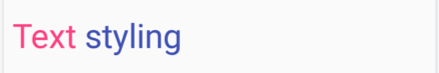
\includegraphics[width=0.5\textwidth,keepaspectratio]{images/span}
    \end{center}
\end{frame}

\begin{frame}[fragile]
    \frametitle{Spannables}
    \begin{minted}{java}
        CharSequence format = "{span} styling"
        SpannableString spannable = new SpannableString("Text");
        spannable.setSpan(ForegroundColorSpan(Color.PINK),
            0, 4, Spannable.SPAN_EXCLUSIVE_EXCLUSIVE);
        CharSequence fullText = Phrase.from(format)
            .put("span", spannable)
            .format()
        spanTextView.setText(fullText);
    \end{minted}
\end{frame}
\begin{frame}[fragile]
    \frametitle{HTML как замена Spannables}
    \begin{minted}{xml}
        <string name="html_example"><b>Text</b> styling</string>
    \end{minted}
    \begin{minted}{java}
        spanTextView.setText(R.string.html_example);
        // or, but note getText usage instead of getString
        spanTextView.setText(getText(R.string.html_example));
    \end{minted}
\end{frame}

\begin{frame}[fragile]
    \frametitle{Фиксированный размер UI-элементов}
    \begin{minted}{xml}
        <!-- Bad -->
        <Button
            android:layout_width="120dp"
            android:layout_height="48dp"
            android:text="@string/do_the_thing_label"/>
        <!-- Good -->
        <Button
            android:layout_width="wrap_content"
            android:layout_height="wrap_content"
            android:text="@string/do_the_thing_label"/>
        <!-- Even better -->
        <Button
            android:layout_width="wrap_content"
            android:layout_height="wrap_content"
            android:minWidth="120dp"
            android:minWHeight="48dp"
            android:text="@string/do_the_thing_label"/>
    \end{minted}
\end{frame}

\begin{frame}[fragile]
    \frametitle{Отсутствие поддержки RTL-локалей}
    \begin{minted}{xml}
        <!-- Bad -->
        <Button
            android:id="@+id/do_the_thing"
            android:layout_width="wrap_content"
            android:layout_height="wrap_content"
            android:layout_marginLeft="16dp"
            android:layout_marginRight="64dp"
            android:text="@string/do_the_thing_label"/>
    \end{minted}
    \begin{minted}{xml}
        <!-- Good -->
        <Button
            android:id="@+id/do_the_thing"
            android:layout_width="wrap_content"
            android:layout_height="wrap_content"
            android:layout_marginStart="16dp"
            android:layout_marginEnd="64dp"
            android:text="@string/do_the_thing_label"/>
    \end{minted}
\end{frame}

\begin{frame}
    \frametitle{Текст в изображениях}
    \begin{center}
        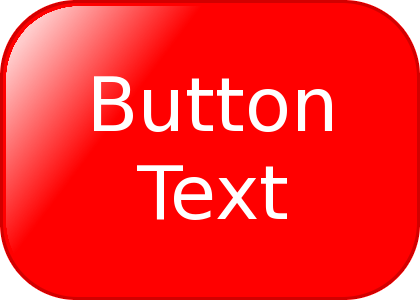
\includegraphics[width=0.3\textwidth,keepaspectratio]{images/button}
    \end{center}
    \begin{itemize}
        \item Заменить на стандартный виджет
        \item Заменить на кастомный виджет
        \item Разбить фон и текст и заменить текст на стандартный виджет
        \item Разбить фон и текст и создать копии текста для разных языков
        \item Создать копии изображения для разных языков
    \end{itemize}
\end{frame}

\begin{frame}
    \frametitle{Локализация с использованием ресурсов}
    \begin{center}
        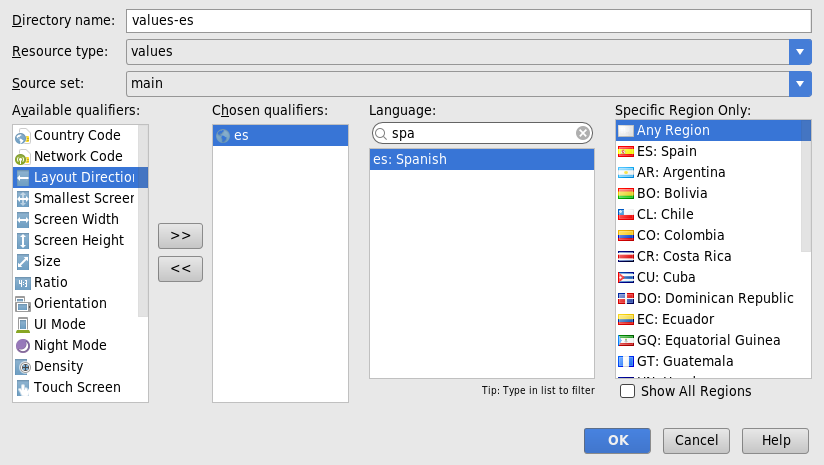
\includegraphics[width=0.7\textwidth,keepaspectratio]{images/resources}
    \end{center}
    \begin{itemize}
        \item UI - \texttt{res/layout/}
        \item Строки - \texttt{res/values/strings.xml}
        \item Изображения \texttt{res/drawable/}
        \item и т. д.
    \end{itemize}
\end{frame}

\begin{frame}
    \frametitle{Локализация с использованием ресурсов}
    \begin{itemize}
        \item Должен быть набор дефолтных ресурсов
        \item Ресурсы со спецификатором локали имеют приоритет над другими ресурсами
            (\texttt{res/drawable-small-land-stylus/ vs. res/drawable-es/})
    \end{itemize}
\end{frame}

\begin{frame}
    \frametitle{Lint}
    \begin{itemize}
        \item \textbf{MissingTranslation} - если строковый ресурс есть в
            дефолтных ресурсах, но отсутствует в ресурсах для конкретной
            локали. Если строка не подлежит переводу, то
            должна быть объявлена с флагом \texttt{translatable=false}
        \item \textbf{ExtraTranslation} - если строковый ресурс есть в ресурсах
			для конкретной локали, но нет в дефолтных.
        \item \textbf{ImpliedQuantity, PluralsCandidate}
    \end{itemize}
\end{frame}

\begin{frame}[fragile]
    \frametitle{Псевдолокализация}
    \begin{minted}{groovy}
        android {
            // ...

            buildTypes {
                debug {
                    pseudoLocalesEnabled true
                }
            }
        }
    \end{minted}
    \begin{itemize}
        \item \textbf{en-XA} - добавляет глифы и увеличивает длину строк
        \item \textbf{ar-XB} - переворачивает строки справо налево и устанавливает
            направление текста справо налево.
    \end{itemize}
\end{frame}

\begin{frame}
    \frametitle{Псевдолокализация}
    \begin{center}
        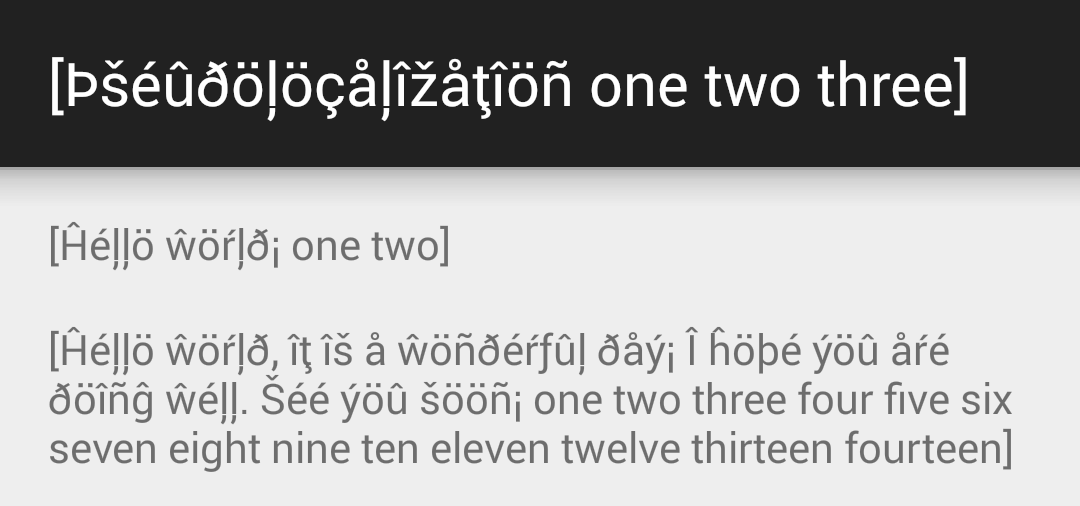
\includegraphics[width=0.7\textwidth,keepaspectratio]{images/pseudolocalization}
    \end{center}
\end{frame}

\begin{frame}
    \frametitle{Ссылки}
    \nocite{*}
    \RaggedRight
    \AtNextBibliography{\scriptsize}
    \printbibliography[heading=none]
\end{frame}

\begin{frame}
    \frametitle{Вопросы?}
\end{frame}

\end{document}
